\documentclass[12pt]{article}
\pdfoutput=1

\usepackage[T1]{fontenc}
%\usepackage[latin9]{inputenc}
\usepackage{verbatim}
\usepackage{float}
\usepackage{amsthm}
\usepackage{amsmath}
\usepackage{amssymb}
\usepackage{graphicx}
%\usepackage{multirow}
\usepackage{color}
\usepackage{url}
\usepackage{caption}
\usepackage{subcaption}
\usepackage{mathtools} 
\usepackage{stackrel} 
%\usepackage[skip=1pt]{caption} % example skip set to 2pt


\newcommand{\LL}{\mathcal{L}}
\newcommand{\E}{\mathbb{E}}
\newcommand{\I}{\mathcal{I}}
\newcommand{\ep}{\varepsilon}
\newcommand{\Z}{\mathbb{Z}}
\newcommand{\GCD}{\mathbf{GCD}}
\newcommand{\XX}{\mathcal{X}}
\newcommand{\SUM}{\text{sum}}
\newcommand{\1}{\mathbf{1}}
\newcommand{\rr}{\textbf{r}}
\newcommand{\ii}{\textbf{i}}
\newcommand{\jj}{\textbf{j}}
\newcommand{\Poisson}{\text{Poisson}}
\newcommand{\II}{\mathcal{I}}
\newcommand{\kk}{\textbf{k}}
\newcommand{\RR}{\mathbb{R}}
\newcommand{\mb}{\mathbf}
\newcommand{\mk}{\mathfrak}
\newcommand{\mc}{\mathcal}
\newcommand*\Bell{\ensuremath{\boldsymbol\ell}}
\newcommand{\TODO}[1]{{\color{red}{[#1]}}}
\newcommand{\revised}[1]{{\color{blue}{#1}}}
\newcommand{\R}{\mathbb{R}}
\newcommand{\M}{\mathcal{M}}
\renewcommand{\P}{\mathbb{P}}
\renewcommand{\L}{\mathcal{L}}

%\newcommand{\SNR}{\ensuremath{\textsf{SNR}}}
\makeatletter

\newcommand{\reals}{\mathbb{R}}
\newcommand{\RL}{\mathbb{R}^L}
\newcommand{\tamir}{x}
\newcommand{\CL}{\mathbb{C}^L}
\newcommand{\RN}{\mathbb{R}^N}
\newcommand{\RNN}{\mathbb{R}^{N\times N}}
\newcommand{\RPP}{\mathbb{R}^{P\times P}}
\newcommand{\CNN}{\mathbb{C}^{N\times N}}
\newcommand{\inner}[1]{\left\langle {#1} \right\rangle}
\newcommand{\hx}{\hat{x}} 
\newcommand{\one}{\mathbf{1}} 
\newcommand{\be}
{\begin{equation}}
\newcommand{\ee}
{\end{equation}}
%\renewcommand{\P}{\mathbb{P}}
\newcommand{\aseq}{\stackrel{a.s.}{=}}
\renewcommand{\P}{\mathrm{Prob}}


\theoremstyle{plain}
\newtheorem{thm}{\protect\theoremname}[section]
\theoremstyle{definition}
\newtheorem{defn}[thm]{\protect\definitionname}
\theoremstyle{remark}
\newtheorem{claim}[thm]{\protect\claimname}
\theoremstyle{plain}
\newtheorem{lem}[thm]{\protect\lemmaname}
\newtheorem*{lem*}{Lemma}
\theoremstyle{remark}
\newtheorem{rem}[thm]{\protect\remarkname}
\theoremstyle{plain}
\newtheorem{corollary}[thm]{\protect\corollaryname}
\theoremstyle{plain}
\newtheorem{conjecture}[thm]{\protect\conjecturename}
\theoremstyle{plain}
\newtheorem{proposition}[thm]{\protect\propositionname}
\providecommand{\claimname}{Claim}
\providecommand{\definitionname}{Definition}
\providecommand{\lemmaname}{Lemma}
\providecommand{\remarkname}{Remark}
\providecommand{\theoremname}{Theorem}
\providecommand{\corollaryname}{Corollary}
\providecommand{\propositionname}{Proposition}
\providecommand{\conjecturename}{Conjecture}

\usepackage{authblk}
\renewcommand*{\Affilfont}{\normalsize}
\setlength{\affilsep}{2em}   % set the space between author and affiliation

\usepackage[margin=3cm]{geometry}

%\allowdisplaybreaks
\numberwithin{equation}{section}


\begin{document}

%\begin{frontmatter}


\title{Multi-target detection with application to cryo-electron microscopy}

\author[a]{Tamir Bendory}
\author[b]{Nicolas Boumal} 
\author[c]{William Leeb}
\author[a,b]{Eitan Levin}
\author[a,b]{Amit Singer}

\affil[a]{The Program in Applied and Computational Mathematics, Princeton University, Princeton, NJ, USA}
\affil[b]{Department of Mathematics, Princeton University, Princeton, NJ, USA}
\affil[c]{School of Mathematics, University of
	Minnesota, Minneapolis, MN, USA }

%\date{}
\maketitle



\begin{abstract}
abstract
%Single-particle cryo-electron microscopy (cryo-EM) has recently joined X-ray crystallography
%and NMR spectroscopy as a high-resolution structural method for biological macromolecules.
%In a cryo-EM experiment, the microscope produces images called micrographs. Projections of the molecule of interest are embedded in the micrographs at unknown locations, and under unknown viewing directions. Standard imaging techniques first locate these projections (detection) and then reconstruct the 3-D structure from them. Unfortunately, high noise levels hinder detection. When reliable detection is rendered impossible, the standard techniques fail. This is a problem especially for small molecules, which can be particularly hard to detect. In this paper, we propose a radically different approach: we contend that the structure could, in principle, be reconstructed directly from the micrographs, without intermediate detection. 
%As a result, even small molecules should be within reach for cryo-EM. To support this claim, we setup a simplified mathematical model and demonstrate how our autocorrelation analysis technique allows to go directly from the micrographs to the sought signals. This involves only one pass over the micrographs, which is desirable for large experiments. 
%We show numerical results and  discuss challenges that lay ahead to turn this proof-of-concept into a competitive alternative to state-of-the-art algorithms.
\end{abstract}

\section{Introduction}

\subsection{Problem formulation} \label{sec:problem_formulation}

We consider the \emph{multi-target detection} problem of recovering a set of $K$ signals that appear 
multiple times at unknown locations in a noisy measurement.
Let $x_1,\ldots,x_K\in\RL$ be the sought signals and let $y\in\RN$ be the observed data, where we assume $N$ is  far larger than $L$. 
Let  $s[i]$ counts the number of signals whose first element is positioned in $y[i]$, each of those  is chosen according to some (possibly unknown) distribution over $\{1,\ldots,K\}$. 
If signal occurrences overlap, they interfere additively. %We think of those events as being rare. 
With additive white Gaussian noise, the measurement model can be written as 
\begin{equation} 
y  =  \sum_{k=1}^K x_k \ast s_k + \varepsilon, \qquad  \varepsilon   \sim \mathcal{N}(0,\sigma^2 I_N),
\label{eq:model}
\end{equation}
where $\ast$ denotes linear convolution, and $s_k[i]$ indicates the number of starting positions of $x_k$ in $y[i]$ so that $s =  s_1+\cdots+s_K$. 
The goal is  to estimate $x_1,\ldots,x_K$ from $y$. % while $s$ is the \emph{nuisance variable} of the problem.
%We name this problem \emph{multi-target detection}.
This idealized setup appears in several scientific applications, including structural biology~\cite{bendory2018toward} (as we detail below), spike sorting~\cite{lewicki1998review}, passive radar~\cite{gogineni2017passive}, and system identification~\cite{ljung1998system}. 

In the low noise regime, a valid strategy is to first detect the signal occurrences in $y$ (that is, estimate $s$), cluster them (that is, separate $s$ into $s_1,\ldots,s_K$), and solve a standard deconvolution problem. Crucially, we focus on the high noise regime, where \emph{reliable detection of signal occurrences is  impossible}~\cite{bendory2018toward,aguerrebere2016fundamental}.
This limitation does not, however, preclude estimation of the signals $x_1,\ldots,x_K$, as we show in this paper. In this setting, we consider  $s_1,\ldots,s_K$  as \emph{nuisance variables}.

In order to recover the signals in the high noise regime, we use autocorrelation analysis.
For any noise level, the autocorrelations of the observation can be estimated to any desired accuracy for large enough $N$. 
This computation is straightforward and requires only one pass over the data.
The underlying principle is to relate the autocorrelations of the observation $y$ to the autocorrelations of $x_1,\ldots,x_K$.
Below we describe two generative models for $s$.  
In these models, the relationship between the autocorrelations of $y$ and those of $x_1,\ldots,x_K$ depend on $s_1,\ldots,s_K$ only through their sums, that is, the total number of occurrences of each signal.
To estimate the signals and occurrence counts from the computed autocorrelations, we solve a nonlinear least-squares (LS) problem as explained in Section~\ref{sec:numerics}. 

The multi-target detection problem  is an instance of  
\emph{blind deconvolution}---a longstanding problem arising in a variety of engineering and scientific applications, such as astronomy, communication, image deblurring, system identification and optics; see~\cite{jefferies1993restoration,shalvi1990new,ayers1988iterative,abed1997blind}, just to name a few. 
Different variants of the blind deconvolution problem have been subject recently to a thorough  analysis~\cite{ahmed2014blind,li2016identifiability,li2016rapid,lee2017blind,ling2017blind,kuo2019geometry}. In clear contrast to multi-target detection, these works focus on the low noise regime and aim at estimating both unknown signals.


%In the low noise regime, one can estimate $s$ and then estimate $x$ by standard deconvolution techniques. However, in the high noise regime, estimating $s$ is impossible---that is, detection is impossible~\cite{bendory2018toward,aguerrebere2016fundamental}. 

\subsection{Generative models}

\paragraph{The well-separated model.}
To guarantee recovery in any noise regime, we require a separation between adjacent signal's occurrences, that is,
\begin{equation}
\textrm{If } s[i] = 1 \textrm{ and } s[j] = 1 \textrm{ for } i \neq j, \textrm{ then } |i - j| \geq 2L-1.
\label{eq:spacing}
\end{equation}
In words: the starting positions of any two occurrences  must be separated by at least $2L-1$ positions, so that their end points are necessarily separated by at least $L-1$ signal-free entries in the data.
%Under the separation condition~\eqref{eq:spacing}, we refer to this model as the \emph{homogeneous well-separated model}. 
In then next section we present a model that alleviates this condition.
%As will be shown next, in a low SNR environment, estimating $s$ is impossible, whereas in some cases estimating $x$ is tractable.

\paragraph{The Poisson model.}

\TODO{For the heterogeneous case.} 

The models we described so far assume a well-separated support. The separation condition can be alleviated by assuming a Poisson process. 
We consider the following observation model. Let $X \in\RL$ be a random vector drawn from some fixed distribution.
Points are chosen in $\{1,\dots,N-L+1\}$ according to a Poisson process with parameter $\gamma (N-L)$. %The parameter $\gamma$ can be thought of as the density of the $X$ in $Y$.
For each point $i$ that is chosen from $1$ to $N-L+1$, a random vector $X$ from the distribution is then placed in $y$, with element $0$ at location $i$, with overlapping vectors being added together. 

If $M_i$ denotes the number of hits at location $i$,  then by definition of the Poisson process $M_i$'s are i.i.d.\ and $M_i \sim \Poisson(\gamma)$. Conditional on the value of $M = (M_1,\dots,M_{N-L+1})$, if we let $X_1^{i},\dots,X_{M_i}^i$ denote the random vectors with position 0 located at $i$, then $X_{k_1}^{i}$ and $X_{k_2}^{i}$ are independent for $k_1 \ne k_2$.
With this notation, we can write each entry as:
%
\begin{align}
%
y[i] = \sum_{j=0}^{L-1} \sum_{k=1}^{M_{i-j}} X_k^{i-j}[j].
%
\end{align}
 
\subsection{Extensions} \label{sec:extensions}

\TODO{multi-dimensions}

The basic model~\eqref{eq:model} can be extended in various ways, some discussed below.
%
%\paragraph{Multi-target detection and clustering with separation.}
%The multi-target detection model can be naturally generalized to the problem of estimating a set of $K$ signals $x_1,\ldots,x_K\in\RL$. Let $s$ be a binary signal satisfying the separation condition~\eqref{eq:spacing}.
%For each $s[i]=1$, a random variable $v_i$ is drawn from some (possibly unknown) distribution over $\{1,\ldots,K\}$. Then, $x_{v_i}$ is placed in $y$
%with element $0$ at location $i$. 
%We refer to this model as \emph{multi-target detection and clustering}.
%
% This model can be written as a mix of blind deconvolution problems
%\begin{equation} 
%y  =  \sum_{k=1}^Kx_k \ast s_k + \varepsilon, \quad  \varepsilon   \sim \mathcal{N}(0,\sigma^2 I_N),
%\end{equation}
%where again $s_i$ is a binary signal, which its non-zero values 
%are the subset of the non-zero values of $s$ associated with $x_i$.
%Generally, we refer to this problem as \emph{multi-target detection and clustering with separation.} 
%An key question in this model is how many signals can be recovered simultaneously. We derive a bound in Section~\ref{sec:heterogeneity} and show a numerical experiment in Section~\ref{sec:numerics}.


\paragraph{The well-separated model with a random signal}
The homogeneous and heterogeneous models can be generalized as follows. 
We let the signal $X\in\RL$ to be a random vector drawn from some fixed distribution. %We observe a random vector $Y\in\R^{N-L+1}$.
For each non-zero element of $s$,  a random vector $X$ from the distribution is then placed in $y$, with element $0$ at location $i$.
If the distribution is a Delta function that this model coincides with the multi-target detection model; if it is a sum of Diracs then it reduces to multi-target detection and clustering.


\section{Motivation: single-particle reconstruction using cryo-electron microscopy}
Cryo-electron microscopy (cryo-EM)  has recently joined X-ray crystallography and nuclear magnetic resonance (NMR) spectroscopy as a high-resolution structural method for biological macromolecules; see for instance~\cite{frank2006three,kuhlbrandt2014resolution,bartesaghi20152}. 
In contrast X-ray and NMR which aggregate information from an ensembles of
particles, single particle cryo-EM produces images of individual particles and thus can, in principle, elucidate multiple  structures.
In addition, it does not require the formation of crystalline arrays of macromolecules.

In a cryo--EM experiment, biological samples are rapidly frozen in a thin layer of vitreous ice.
The microscope produces a 2-D tomographic image of the samples embedded in the ice, called a \emph{micrograph}. Each micrograph contains tomographic projections of the samples at unknown locations and under unknown viewing directions. The goal is to construct 3-D models of the molecular structure from the micrographs. 
Importantly, to keep radiation damage within acceptable bounds, the dose must be kept low, leading to high noise levels.

All contemporary methods in the field split the reconstruction procedure into two main  stages.
The first stage consists in extracting the  particle projections from the micrographs. This stage is called \emph{particle picking}. The second stage aims to construct a 3-D model of the molecular structure from these projections. The quality of the reconstruction eventually hinges on the quality of the particle picking stage.
Crucially, it can be shown that reliable detection of individual particles is impossible below a certain critical SNR. This fact has been recognized early on by the cryo-EM community. 
Particularly, in~\cite{henderson1995limitations,glaeser1999electron}, it was established that particle picking is impossible for molecules below a certain weight (below $\sim$50 kDa). 
%The unique issues raised by small particles have been mitigated by recent technological advances in the field, including the use of Volta phase plates~\cite{khoshouei2017cryo,liang2017phase} and scaffolding cages~\cite{liu2018nearatomic}.
%Despite this progress, detecting small molecules in the micrographs remains a challenge.

Another potential pitfall of particle picking pertains to \emph{model bias}, whose importance in cryo-EM was stressed by a number of authors~\cite{shatsky2009method,vanheel1992correlation,henderson2013avoiding,vanheel2013finding}. In the classical ``Einstein from noise'' experiment, multiple realizations of pure noise are aligned to a picture of Einstein using template matching and then averaged. In~\cite{shatsky2009method}, it was shown that the averaged noise rapidly becomes remarkably similar to the Einstein template. In the context of cryo--EM, this experiment exemplifies how prior assumptions about the particles may influence the reconstructed structure. This model bias is common to all particle picking methods based on template matching. %In our approach, no templates or human intervention are required, thus significantly reducing concerns about model bias. %

A recent work of the authors suggests to bypass the particle picking stage and  reconstruct the 3-D structure directly from the micrograph~\cite{bendory2018toward}.
In that paper, it was shown that---at least in principle---the limits particle picking imposes on molecule size do not necessarily  translate into limits on particle reconstruction.
The principle mathematical tool is  \emph{autocorrelation analysis}, described in detail in Section~\ref{sec:AC_analysis}.
This goal of  the current paper is to provide a theoretical justification and numerical support  for the method proposed in~\cite{bendory2018toward}.  
In this context, the  models described above serve  as  an abstraction of the cryo-EM problem: the random signal $X$ discussed in Section~\ref{sec:extensions} can be thought of as 2-D random tomographic projections of the 3-D structure 
taken according to some unknown distribution of the particles within the ice.

% A similar abstraction has been proven itself to be useful in a similar context as described in the next section. 

We mention that~\cite{bendory2018toward} was not the first paper to employ autocorrelation analysis to cryo-EM. 
Zvi Kam~\cite{kam1980reconstruction} first proposed autocorrelation analysis for \mbox{3-D} reconstruction, under the assumption of perfect particle picking: his method used autocorrelations of the picked, perfectly centered, particles. His method has been extended and employed by in X-ray free electron lasers and cryo-EM; see for instance~\cite{liu2013three,kurta2017correlations,levin20173d,von2018structure}.  
In order to investigate the computational and statistical properties of Kam's method, a series of papers have studied a simplified model, 
called   \emph{multi-reference alignment}~\cite{bandeira2014multireference,bendory2017bispectrum,bandeira2017optimal,perry2017sample,bandeira2017estimation,abbe2017multireference}.
We follows the same line of research by considering the multi-target detection and clustering  as an abstraction to the application of reconstructing 3-D structures directly from the micrograph as proposed in~\cite{bendory2018toward}.

%\subsection{Principle mathematical tool: autocorrelation analysis.}



%Our problem can be interpreted as a special case of the \emph{system identification} problem. Similarly to~\eqref{eq:model}, the
%forward model takes the form
%%
%\begin{math}
%%
%y = x\ast w + \varepsilon,  
%%
%\end{math} 
%%
%where $x$ is the unknown signal (the system's impulse response), $w$ is an unknown (often random) input sequence, and $\varepsilon$ is an additive noise.
%The goal of this problem is to estimate $x$, usually referred to as ``identifying the system.'' The question of identifiability of $x$ under this observation model is addressed for certain Gaussian and non-Gaussian $w$ in~\cite{benveniste1980robust,kormylo1983identifiability}. In the special case where $w$ is binary and satisfies our separation condition, we recover our model. 
%
%Likelihood-based methods estimate $x$ as the maximizer of some function $f(x | y)$, where $f$ is derived from the likelihood function of $x$ given the observed signal $y$.  
%If some prior is assumed on $x$, then $f(x|y)$ can be taken to be the posterior distribution of $x$ given the data; this is the simplest form of Bayesian inference.
%Methods based on such formulations are popular nowadays in cryo-EM; see for instance~\cite{sigworth1998maximum,scheres2012relion}. 
%Optimizing the function $f(x|y)$ exactly is often intractable, and thus heuristic methods are used instead. One proposed technique is to use Markov Chain Monte Carlo (MCMC)~\cite{cappe1999simulation}. 
%In special cases, including the case where $w$ is binary, expectation maximization (EM) has been used~\cite{cappe1999simulation}. The EM method for discrete $w$ is based on a certain ``forward-backward'' procedure used in hidden Markov models~\cite{rabiner1989tutorial}. However, the complexity of this procedure is superlinear in $N$, and therefore its usage is limited for big data sets. 
%
%Because likelihood methods are computationally expensive, methods based on recovery from moments have also been previously used for system identification. Methods based on the third- and fourth-order moments are described and analyzed in~\cite{lii1982deconvolution,giannakis1989identification,tugnait1984identification}. Building on such ideas, we focus on an autocorrelation analysis for~\eqref{eq:model}. 


%
%\section{The detection limit} \label{sec:detectionlimit}
%
%In the low SNR regime---even if $x$ is known---estimating the binary sparse signal $s$ is impossible, that is, one cannot reliably detect occurrences of $x$ in the micrograph $y$.
%To support this claim, we consider a strictly simpler problem: suppose an oracle identifies for us one interval of length $L$ in the micrograph that either contains a full signal occurrence (plus noise), or contains just noise. Our task is to determine which one it is, that is, to determine whether the corresponding entry of $s$ is 0 or 1.
%The oracle further provides the signal $x$, the probability $q$ that  the interval contains signal, and the noise variance $\sigma^2$. 
%
%This decision problem can be abstracted as follows: We have two known vectors $\theta_0 = x$ and $\theta_1 = 0$ in $\mathbb{R}^L$. There is a random variable $\eta$ taking values 0 or 1 with probabilities $q$ and $1-q$, respectively. We observe a random vector $X \in \mathbb{R}^L$ (an extract of the micrograph) with the following distribution: if $\eta = 0$, then $X \sim \mathcal N(\theta_0,\sigma^2I_L)$ and if $\eta = 1$, then $X \sim \mathcal N(\theta_1,\sigma^2I_L)$. 
%
%We observe $X$, and our task is to estimate $\eta$. How reliably can this be done? If $q \geq 1/2$, the constant estimator $\hat{\eta} = 0$ is correct with probability $q$; likewise, if $q \leq 1/2$, the constant estimator $\hat{\eta} = 1$ is correct with probability $1-q$. The question is, can we do better than this?  We prove that, as $\sigma \to \infty$, the answer is no. The result is proved in Appendix~\ref{sec:proof_two_gauss}.
%
%\begin{proposition} \label{prop:two_gauss}
%	For any deterministic estimator $\hat{\eta }$ of $\eta$,
%	\begin{equation}
%	\lim_{\sigma \to \infty} \P[ \hat{\eta} = \eta  ] \leq \max(q, 1-q);
%	\end{equation}
%	that is: as the SNR deteriorates, the probability of success is no better than random chance.
%\end{proposition}
%
%Proposition~\ref{prop:two_gauss} implies that in order to estimate the signal at low SNR we must consider methods that aim to estimate the signal $x$ directly, without estimating the nuisance variable $s$ as an intermediate step.
%In the next sections, we consider autocorrelation analysis for that purpose.


\section{Autocorrelation analysis} \label{sec:AC_analysis}

%
%In order to recover the signal, we employ autocorrelation analysis. The underlying principle is to relate the autocorrelations of the observation to the autocorrelations of the signal without trying to detect individual signal occurrences (i.e., the signal $s$).
%In the models described above, for any noise level, these autocorrelations can be estimated to any desired accuracy in the limit of $N\to\infty$. 
%The autocorrelations of the observation are straightforward to compute and require only one pass over the data. After estimation of the density of particles in the micrographs, these directly yield estimates for the mixed autocorrelations of the signals. To estimate the signals them from their estimated autocorrelations, we solve a nonlinear inverse problem as explained in Section~\ref{sec:numerics}. 


Let $Z\in \R^m$ be a random signal drawn from some fixed distribution.  The autocorrelation of order $q = 1, 2, \ldots$ is given for any integer shifts $\ell_1, \ldots, \ell_{q-1}$ by
\begin{equation}
a_Z^q[\ell_1,\ldots,\ell_{q-1}]   = \E\left\{\frac{1}{m} \sum_{i=-\infty}^{\infty} Z[i]Z[i+\ell_1]\cdots Z[i+\ell_{q-1}]\right\},
\label{eq:ac_general}
\end{equation}
where the expectation is taken with respect to the distribution of $Z$. The indexing of $Z$ out of the range $0, \ldots, m-1$ is zero-padded.
Explicitly, the first-, second- and third-order autocorrelations are given by: 
\begin{align} 
a_Z^1 & = \frac{1}{m} \sum_{i=0}^{m-1} \E\left\{
Z[i]\right\}, \nonumber\\
a_Z^2[\ell] & = \frac{1}{m} \sum_{i = \max\{0, -\ell\}}^{m-1 + \min\{0, -\ell\}} \E\left\{Z[i]Z[i+\ell]\right\},\\
a_Z^3[\ell_1,\ell_2] & = \frac{1}{m} \sum_{i = \max\{0, -\ell_1, -\ell_2\}}^{m-1 + \min\{0, -\ell_1, -\ell_2\}} \E\left\{Z[i]Z[i+\ell_1]Z[i+\ell_2]\right\}.  \nonumber \label{eq:ac_special}
\end{align}
The autocorrelation functions have symmetries. Specifically, $$\E\left\{a_Z^2[\ell]\right\} = \E\left\{a_Z^2[-\ell]\right\},$$ and \TODO{to verify}
$$\E\left\{a_Z^3[\ell_1,\ell_2]\right\} = \E\left\{a_Z^3[\ell_2,\ell_1]\right\}=\E\left\{a_Z^3[-\ell_1,\ell_2-\ell_1]\right\}.
$$
For our purposes, this will be applied both to $x$ (of length $L$) and to $y$ (of length $N$).

Under the separation condition, the relation between autocorrelations of the micrograph and those of $X$ is particularly simple, as we now show. It is useful to introduce some notation: let $M$ denote the number of occurrences of $X$ in $y$ (that is, the number of 1's in $s$), and let
\begin{equation}
\gamma  = \frac{M L}{N}
\label{eq:gamma}
\end{equation}
denote the density of $X$ in $y$ (that is, the fraction of entries of $y$ occupied by occurrences of $X$.) 
In this section, we assume the separation condition~\eqref{eq:spacing} that  imposes $\gamma\leq\frac{L}{2L-1}\approx 1/2$. In Section~\ref{sec:poisson} we show that the autocorrelations in the Poisson model are equivalent to  those presented in this section.

For shifts in $0, \ldots, L-1$, the autocorrelation functions of $y$ depend on the corresponding autocorrelations of $x$, the noise level $\sigma$ and the support signal $s$. Importantly, under the separation condition~\eqref{eq:spacing}, the dependency on $s$ is only through the density $\gamma$.
We consider the asymptotic regime where $\gamma$ remains constant; that is, as $N$ goes to infinity, $M$ also goes to infinity at the same rate (in other words, as we see an increasingly large observation, it contains increasingly many signal occurrences, with constant signal density). In that regime, the law of large numbers can be used to show the following statement:
\begin{equation} \label{eq:mean_micrograph}
\lim_{N\to\infty} a_y^1  \aseq \gamma a_{X}^1,
\end{equation}
\TODO{ should is be $\E\left\{a_{X}^1\right\}$?} where equality holds almost surely (a.s.), meaning it holds with probability one.
The randomness is over the Gaussian noise $\varepsilon$; $s$ may be deterministic.
Thus, given enough data, if $\gamma$ is known, we can estimate $a_{X}^1$ from $y$. We show in Section~\ref{sec:theory_homogeneous} how to estimate $\gamma$ as well in the homogeneous model. 

We have a similar observation for the second-order autocorrelation: $a_y^2[\ell]$ computes the correlation between $y$ and a copy of $y$ shifted by $\ell$ entries. Considering $\ell$ only in the range $0, \ldots, L-1$, one can see that any given occurrence of $x$ in $y$ is only ever correlated with itself, and never with another occurrence. As a result,
\begin{equation}
\lim_{N\to\infty} a_y^2[\ell]  \aseq \gamma a_{X}^2[\ell] + \sigma^2\delta[\ell],
\label{eq:ac2_micrograph}
\end{equation}
%\begin{equation}
%\lim_{N\to\infty} a_y^2[\ell]  \aseq \gamma \E\left\{a_{X}^2[\ell]\right\} + \sigma^2\delta[\ell],
%\label{eq:ac2_micrograph}
%\end{equation}
for $\ell = 0, \ldots, L-1$, where $\delta[\ell]$ equals one for $\ell=0$ and zero otherwise. The last part captures the autocorrelation of the noise. Notice that, even if $\sigma$ is unknown, entries $\ell = 1, \ldots, L-1$ still provide useful information about $a_{X}^2[\ell]$.

Along the same lines, one can establish a relation for third-order autocorrelations:
\begin{equation}
 \label{eq:ac3_micrograph}
\lim_{N\to\infty} a_y^3[\ell_1,\ell_2] \aseq \gamma a_{x}^3[\ell_1,\ell_2]  + \sigma^2\gamma a_{X}^1  \big(\delta[\ell_1,0]+\delta[0,\ell_2]
+\delta[\ell_1,\ell_2]\big),
\end{equation}
for $\ell_1,\ell_2 = 0, \ldots, L-1$, where $\delta[\ell_1,\ell_2]:=\delta[\ell_1-\ell_2]$.
Here too, few entries are affected by $\sigma$ in the limit.

%
%Computing the autocorrelations of the micrograph is straightforward. The natural question, treated next, is whether one can recover $x$ from them.


\section{Theory}

\subsection{Theory for the homogeneous case} \label{sec:theory_homogeneous}
In this section, we derive some theoretical results for the homogeneous case. \TODO{Note: I am using terms interchangeably}
 
A signal is determined uniquely by its second- and third-order autocorrelations. Indeed, assuming $z[0]$ and $z[L-1]$ are nonzero (otherwise, redefine the length of the signal), we can recover $z$ explicitly using this identity for $k = 0, \ldots, L-1$:
%
\begin{equation}
%
z[k]  = \frac{z[0]z[k]z[L-1]}{z[0]z[L-1]} = \frac{a_z^3[k,L-1]}{a_z^2[L-1]}.
\label{eq-uniqueness}
%
\end{equation}
This proves the following useful fact:
\begin{proposition} \label{prop:uniqueness}
	%
	A signal $z\in\RL$ is determined uniquely from  $a_z^2$ and $a_z^3$.
\end{proposition}

A couple of remarks are in order. First, \eqref{eq-uniqueness} is not numerically stable: if $z[0]$ or $z[L-1]$ are close to 0, recovery of $z$ is sensitive to errors in the autocorrelations. In practice, we recover $z$ by fitting it to its autocorrelations using a nonconvex least-squares (LS) procedure, which is empirically more robust to additive noise; we have observed similar phenomena for related problems~\cite{bendory2017bispectrum,boumal2017heterogeneous,abbe2017multireference}.
%Second, note that the second-order autocorrelation is not by itself sufficient to determine the signal uniquely. %~\cite{beinert2015ambiguities,bendory2017fourier}.

The observed moments $a_y^1,a_y^2$ and $a_y^3$ of $y$ do not immediately yield the moments of the signal $x$, as seen by~\eqref{eq:mean_micrograph},~\eqref{eq:ac2_micrograph} and~\eqref{eq:ac3_micrograph}; rather, the two are related by the noise level $\sigma$ and the ratio $\gamma$. We will show, however, that $x$ is still determined by the observed moments of $y$.

First, we observe that if the noise level $\sigma$ is known, generally, one can estimate $\gamma$ from the first two moments of the micrograph. The proof is provided in Appendix~\ref{sec:proof_prop_gamma}.

\begin{proposition} \label{prop:gamma}
	Let $\sigma > 0$ be fixed and assume that the separation condition~\eqref{eq:spacing} holds. If the mean of $x$ is nonzero, then 
	\begin{equation}
	\gamma  \aseq \lim_{N \to \infty}\frac{L (a^1_y)^2}{a_y^2[0] + 2\sum_{\ell = 1}^{L-1}a_y^2[\ell]-\sigma^2}.
	\end{equation}
\end{proposition}

Using third-order autocorrelation information of $y$, both the ratio $\gamma$ and the noise $\sigma$ are determined. For the following results, when we say that a result holds for a ``generic'' signal $x$, we mean that the set of signals which cannot be determined by these measurements
has Lebesgue measure zero. 
In particular, this means that we can recover
almost all signals with the given measurements. The proof is provided in Appendix~\ref{sec:proof_prop_gamma_sigma}.

\begin{proposition} \label{prop:gamma_sigma}
	Assume $L \geq 3$ and assume that the separation condition~\eqref{eq:spacing} holds. 
	In the limit of $N\to \infty$, the observed autocorrelations $a_y^1,a_y^2$ and  $a_y^3$ determine the ratio $\gamma$ and noise level $\sigma$ uniquely for a generic signal $x$. If $\gamma > \frac{1}{4}$, then this holds for any signal $x$ with nonzero mean. 
\end{proposition}

From Propositions~\ref{prop:uniqueness} and~\ref{prop:gamma_sigma} we   deduce the following:
\begin{corollary}
	In the limit of $N\to \infty$ and under the separation condition~\eqref{eq:spacing}, the signal $x$, the ratio $\gamma$, and the noise level $\sigma$ are determined from the first three autocorrelation functions of $y$ if either the signal $x$ is generic or $x$ has nonzero mean  and $\gamma > \frac{1}{4}$.
\end{corollary}

As a side note, under the separation condition, the length $L$ of the signal can also be determined from the autocorrelations in the asymptotic regime, by inspection of the support of $a_y^2$.


\subsection{Equivalence between the autocorrelations of under the separation and the Poisson process \TODO{?}} \label{sec:poisson}

In this section we omit the affect of the noise as it remains the same for the well-separated model. We aim to show that the moments of 

Let us denote by $m_Y^q$ the moments of $Y$:
%
\begin{align}
%
m_X^1[i] &= \E X[i], \quad 0 \le i \le L-1,   \nonumber\\ 
m_X^2[i,j] &= \E X[i] X[j], \quad 0 \le i,j \le L-1, \\ 
m_X^3[i,j,k] &= \E X[i] X[j] X[k], \quad 0 \le i,j,k \le L-1. \nonumber
\end{align}
%
Note that 
\begin{align}
a_X^1 &= \frac{1}{L}\sum_{i=0}^{L-1}m_X^1[i], \nonumber \\
a_X^2[\ell] &= \frac{1}{L}\sum_{i=0}^{L-1}m_X^2[i,i+\ell], \\
a_X^3[\ell_1,\ell_2] &= \frac{1}{L}\sum_{i=0}^{L-1}m_X^3[i,i+\ell_1,i+\ell_2]. \nonumber
\end{align}


In the following,  we show that the moments of the observed data under the Poisson process can be written in terms of the autocorrelations of the well-separated model.

\begin{proposition} \label{prop:poisson}
    For any $i$,  the moments under the Poisson process are equal to 
    \begin{align}
    m_y^1[i] &= \gamma L a_X^1 \nonumber \\
    m_y^2[i,i+\ell] &= (\gamma a_X^1)^2 + \gamma a_X^2[\ell],\quad \ell=0,\ldots,L-1, \\
    m_y^3[i,i+\ell_1,i+\ell_2] &= (\gamma a_X^1)^3 + \gamma a_X^1  \cdot ( \gamma a_X^2[\ell_1] + \gamma a_X^2[\ell_2] + \gamma a_X^2[\ell_2-\ell_1]) + \gamma a_X^3[\ell_1,\ell_2]. \nonumber  
    \end{align}
\end{proposition}


\begin{corollary} \TODO{re-write}
	From the first three moments of the Poisson process model, one can recover the first three moments from the strongly-separated model.
\end{corollary}



\subsection{Autocorrelations in higher dimensions} \label{sec:high_dimensions}

Autocorrelations in $d$ dimensions is defined for  $\ell_1,\ldots,\ell_{q-1}\in\mathbb{Z}^d$  as 
\begin{equation}
a_Z^q[\ell_1,\ldots,\ell_{q-1}]   = \E\left\{\frac{1}{m^d} \sum_{i\in\mathbb{Z}^d} z[i]z[i+\ell_1]\cdots z[i+\ell_{q-1}]\right\}.
\label{eq:ac_d_dimension}
\end{equation}
Interestingly, for dimensions greater than one almost all deterministic (that is, the distribution of $Z$ is a Delta function) signals are determined uniquely from their second-order autocorrelation, up to two symmetries: sign (or phase for complex signals) and reflection through the origin (with conjugation in the complex case)~\cite{hayes1982reconstruction}. 
If the mean of signal is available and non-zero, the sign symmetry can be resolved. However, determining the reflection symmetry still requires additional information, beyond the second-order autocorrelation.
The case of 1-D signals is essentially different: generally there are $2^{L-2}$ signals with the same second-order autocorrelation (after eliminating  symmetries)~\cite{beinert2015ambiguities,bendory2017fourier}. 


This uniqueness result for multi-dimensional signals (especially for 2-D images) is the basis of a popular imaging technique called coherent diffraction imaging (CDI). In CDI, an object is
illuminated with a coherent wave, and the far field diffraction
intensity pattern  is measured, corresponding object's Fourier magnitude~\cite{miao1999extending,shechtman2015phase}. 
If the support of the object is known and less than half of the support of the measured signal, then the data is equivalent to the second-order autocorrelation. The computational problem of recovering the signal is usually referred to as \emph{phase retrieval} or \emph{phase problem}.
Albeit the uniqueness result, recently it has been shown that, at least for 2-D images, the problem is  ill-conditioned~\cite{barnett2018geometry}. That is, there exist different images whose second-order autocorrelation agree up to machine precision. 

\subsection{How many signals can be recovered in the heterogeneous model?}
\label{sec:heterogeneity}

In the heterogeneous models, the autocorrelation of $K$ signals are mixed together. To this end, we count how many equations the first three autocorrelations provide, after omitting symmetries. While we do not provide a rigorous proof, it was shown in similar problems that number of equations captures exactly how many signals can be decomposed for a mix of their autocorrelations~\cite{bandeira2017estimation}.

\TODO{Probably should be re-written}
Clearly, the first-order autocorrelation provides us one equation. For second-order autocorrelations, notice  that $a_y^2[\ell]$ suffers no noise-induced bias for $\ell$ in $1$ to $L-1$. Thus if $\sigma$ is known we obtain $L$ equations, while if not we omit $\ell = 0$. This has the practical effect that we need not know $\sigma$ to make sense of the computed quantities, while loosing one one equation. 
Likewise, for third-order autocorrelations, $a_y^3[\ell_1, \ell_2]$ for $0 \leq \ell_1, \ell_2 \leq L-1$ such that $\ell_2 \leq \ell_1$ includes all relevant entries for our purpose (this accounts for symmetries): $\frac{(L+1)(L+2)}{2}-2$ in total. 
If we further exclude any such that $\ell_1, \ell_2$ or $\ell_1 - \ell_2$ are zero to avoid the need to estimate $\sigma$---there are $\frac{(L-1)(L-2)}{2}$ remaining entries. 
Hence, if $\sigma$ is known we have 
\begin{align*}
1 + L + \frac{(L+1)(L+2)}{2}-2 = \frac{1}{2} L (L+5)
\end{align*}
and if it unknown
\begin{align*}
1 + (L-1) + \frac{(L-1)(L-2)}{2} = \frac{1}{2} L (L-1) + 1
\end{align*}
coefficients in total. Since we aim to estimate $KL$ parameters (for the $K$ signals of length $L$) plus $K$ parameters (for the densities $\gamma_k$), an absolute upper bound on $K$  is
\begin{equation}
K\leq \frac{L(L+5)}{2(L+1)},
\end{equation}
\begin{align*}
K \leq \frac{ L (L-1) + 1}{2(L+1)}.
\end{align*}
Thus, we conjecture that approximately $L/2$ signals can be decomposed from  the first three mixed autocorrelations.


\section{Algorithms and numerical experiments} \label{sec:numerics}

The technique we advocate allows recovery of a signal hidden in noisy micrographs without detecting the location  of the signals embedded in these micrographs. To illustrate the underlying principles of the method, we present several numerical examples. The code to generate all figures is publicly available in \url{https://github.com/PrincetonUniversity/BreakingDetectionLimit}.

In the first experiment, we estimated 
an 50-by-50 pixel image of Einstein with mean zero from a growing number of micrographs, each of size $4096\times 4096$ pixels. Each micrograph contains, on average, 700 occurrences of the target image at random locations. 
Thus, about 10\% of each micrograph contains signal. The micrographs are contaminated with additive white Gaussian noise with standard deviation $\sigma=3$,  corresponding  to SNR = $\frac{M\|x\|_F^2} {\sigma^2N} \approx1/370$. This high noise level is illustrated in Figure~\ref{fig:micro_example}. 
To simplify the experiment, we assume the number of signal occurrences and the noise standard deviation are known. Micrographs are generated such that any two occurrences are always separated by at least 49 pixels in each direction in accordance with the separation condition~\eqref{eq:spacing}. 

We compute the average second-order autocorrelation of the micrographs. This is a particularly simple computation which can be efficiently executed with a fast Fourier transform (FFT) in parallel.  
Given the noise level and number of image repetitions, the second-order autocorrelation of the image can be easily deduced from~\eqref{eq:ac2_micrograph}.  Then, to estimate the target image, we resort to a standard phase retrieval algorithm called relaxed-reflect-reflect (RRR)~\cite{elser2017rrr}, initialized randomly.
Relative error is measured as the ratio of the root mean square error to the norm of the ground truth (square root of the sum of squared pixel intensities).

Figure~\ref{fig:Einst_example} shows several estimated images for a growing number of micrographs. 
Figure~\ref{fig:error_per_micro} %(see appendix)
presents the normalized recovery error as a function of the amount of data available.  This is computed after fixing the reflection symmetries (see Section~\ref{sec:AC_analysis}). As evidenced by these figures, the ground truth image can be estimated increasingly well from increasingly many micrographs, without particle picking.

\begin{figure}[t]
	\centering
	\begin{subfigure}[h]{0.33\linewidth}
		\centering
		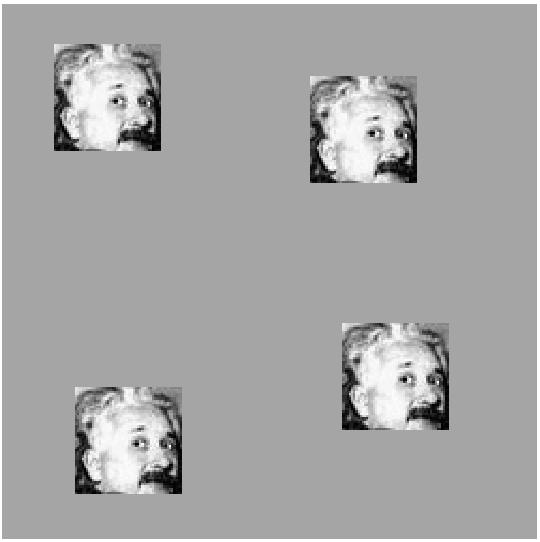
\includegraphics[width=.8\linewidth]{micrograph_Einstein_example_clean}
		\caption{$\sigma = 0$}
	\end{subfigure}%
	\begin{subfigure}[h]{0.33\linewidth}
		\centering
		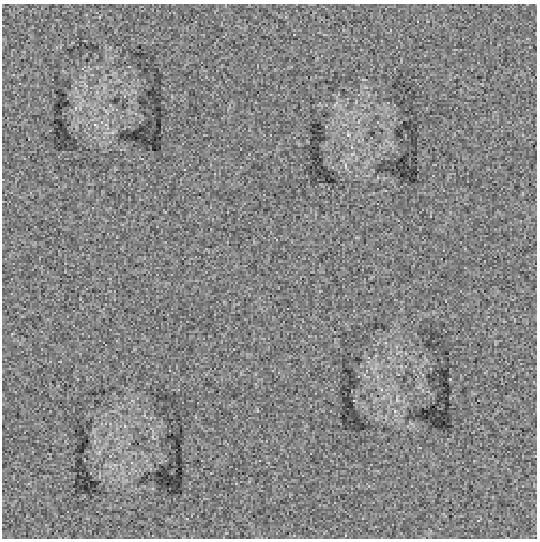
\includegraphics[width=.8\linewidth]{micrograph_Einstein_example_s05}
		\caption{$\sigma = 0.5$}
	\end{subfigure}
	\begin{subfigure}[h]{0.33\linewidth}
		\centering
		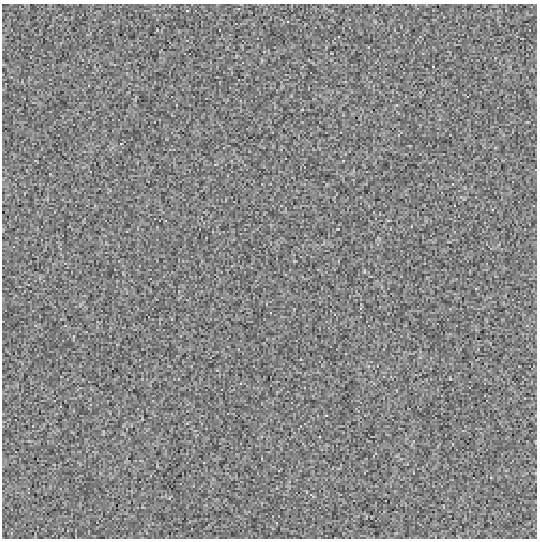
\includegraphics[width=.8\linewidth]{micrograph_Einstein_example_s3}
		\caption{$\sigma = 3$}
	\end{subfigure}
	\caption{\label{fig:micro_example} Example of micrographs of size $250\times 250$ with additive white Gaussian noise of variance $\sigma^2$ for increasing values of $\sigma$. Each micrograph contains the same four occurrences of a $50 \times 50$ image of Einstein. In panel (c), the noise level is such that it is very challenging to locate the occurrences of the planted image. In fact, it can be shown that at low SNR, reliable detection of individual image occurrences is impossible, even if the true image is known. By analogy to cryo-EM, this depicts a scenario where particle picking cannot be done.}
	%\vspace{-8pt} 	
\end{figure}


\begin{figure}[t]
	\centering
	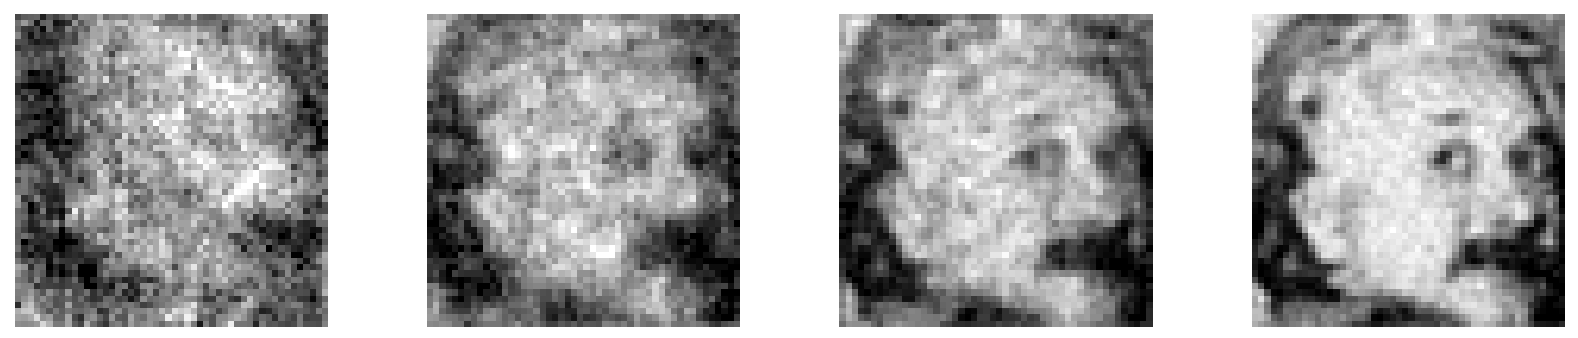
\includegraphics[width=1\linewidth]{Einstien_progress_examples}
	\caption{\label{fig:Einst_example} Recovery of Einstein from micrographs at noise level $\sigma = 3$ (see Figure~\ref{fig:micro_example}(c)). Averaged autocorrelations of the micrographs allow to estimate the power spectrum of the target image. This does not require particle picking. A phase retrieval algorithm (RRR) produces the estimates here shown, initialized randomly. Estimates are obtained from $2\times 10^2,2\times 10^3,2\times 10^4,2\times 10^5$ micrographs (growing across panels from left to right) of size $4096\times 4096$, each containing $700$ image occurrences on average.}	
	%	\vspace{-8pt} 
\end{figure}


 Appendix~\ref{sec:numeric_details} provides additional details on the experiments. 

\begin{figure}[h]
	\centering
	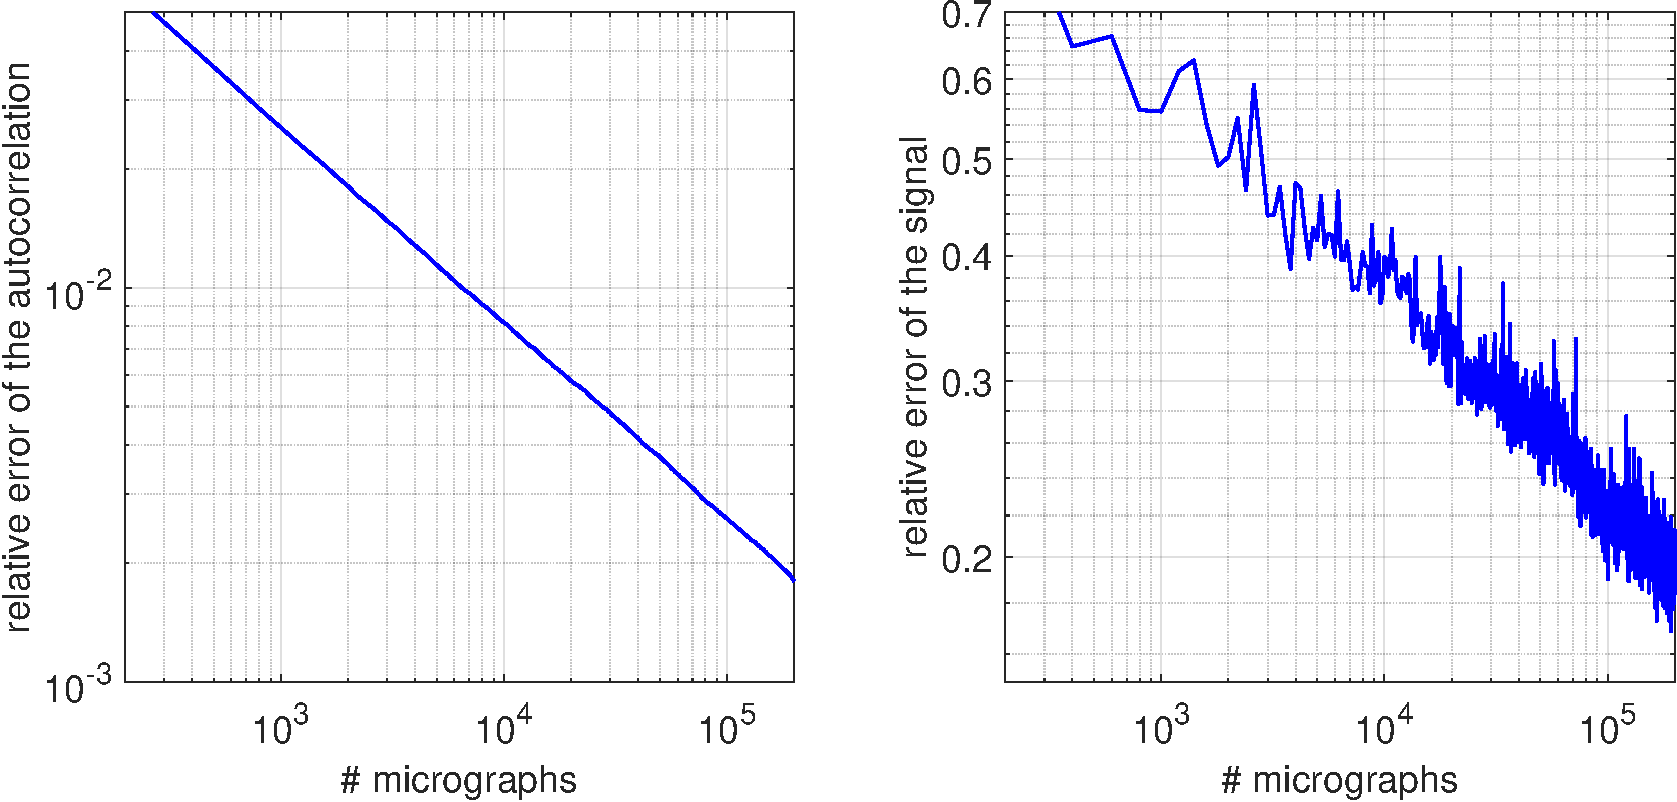
\includegraphics[width=.8\linewidth]{Einstein_recovery_error_combined}
	\caption{\label{fig:error_per_micro}Relative error curves for the experiment of Figure~\ref{fig:Einst_example}.}
\end{figure}


In practice, we do not expect to know $\gamma$ and maybe not even $\sigma$


\paragraph{Numerical experiment with three 1-D signals.}


For the 1-D experiment depicted in Figure~\ref{fig:1Dheterosignals}, we fix $K = 3$ signals of length $L = 21$. Following the forward model described at the beginning of this section, we generate an observation $y$ of length $12.3 \cdot 10^9$. Each of the three signals appears, respectively (and approximately), $30.0 \cdot 10^6$, $20.0 \cdot 10^6$ and $10.0 \cdot 10^6$ times in $y$ for a total of exactly $60 \cdot 10^6$ occurrences, such that at least $L-1$ zeros separate any two occurrences of any signals. 
This is done by randomly selecting $60 \cdot 10^6$ placements in $y$, one at a time with an accept/reject rule based on the separation constraint and locations picked so far. For each placement, one of the three signals is picked at random according to the proportions $1/2, 1/3, 1/6$. Then, i.i.d.\ Gaussian noise with mean zero and standard deviation $\sigma = 3$ is added, to form the observed $y$. The resulting SNR of $y$
% sqrt((m_want*sum(X.^2)')/(sigma^2*n))
is about 1/9.


This is enough noise to make cross-correlations of $y$ even with the true signals display peaks at essentially random locations, uninformative of the actual locations of the signal occurrences. Thus, we contend that it would be difficult for any algorithm to locate the signal occurrences, let alone to classify them according to which signal appears where.

%\TODO{TB: I would place the equation counting argument in the theory section in the paragraph of open questions (I marked th place)}
%
Given the observation $y$, we proceed to compute the autocorrelations. The first-order autocorrelation is straightforward. For second-order autocorrelations, notice from equation~\eqref{eq:data_ac} that $a_y^2[\ell]$ suffers no noise-induced bias for $\ell$ in $1$ to $L-1$. Thus, we omit $\ell = 0$, which has the practical effect that we need not know $\sigma$ to make sense of the computed quantities. Likewise, for third-order autocorrelations, $a_y^3[\ell_1, \ell_2]$ for $0 \leq \ell_1, \ell_2 \leq L-1$ such that $\ell_2 \leq \ell_1$ includes all relevant entries for our purpose (this accounts for symmetries), and we further exclude any such that $\ell_1, \ell_2$ or $\ell_1 - \ell_2$ are zero to avoid the need to estimate $\sigma$---there are $\frac{(L-1)(L-2)}{2}$ remaining entries. We have
\begin{align*}
1 + (L-1) + \frac{(L-1)(L-2)}{2} = \frac{1}{2} L (L-1) + 1
\end{align*}
coefficients in total. Since we aim to estimate $KL$ parameters (for the $K$ signals of length $L$) plus $K$ parameters (for the densities $\gamma_k$), an absolute upper bound on $K$ (simply to ensure we have at least as many equations as we have unknowns) is
\begin{align*}
K(L+1) \leq \frac{1}{2} L (L-1) + 1.
\end{align*}
Thus, $(L-1)/2$ (up to a small approximation) is an absolute upper limit on $K$ (compare with~\cite{boumal2017heterogeneous,bandeira2017estimation}). \TODO{The last paragraph can be removed}
In practice, the autocorrelations are computed on disjoint segments of $y$ of length $100\cdot10^6$ and added up, without correction for the junction points. Segments are handled sequentially on a GPU, as GPUs are particularly well suited to execute simple instructions across large vectors of data. If multiple GPUs are available, segments can of course be handled in parallel.

Having computed the moments of interest, we now estimate signals $x_1, \ldots, x_K$ and coefficients $\gamma_1, \ldots, \gamma_K$ which agree with the data. We choose to do so by running an optimization algorithm on the following nonlinear least-squares problem:
\begin{multline}
\min_{\substack{\hat x_1, \ldots, \hat x_K \in \R^{W} \\ \hat \gamma_1, \ldots, \hat \gamma_K > 0}} w_1 \left( a_y^1 - \sum_{k=1}^K \hat \gamma_k a_{\hat x_k}^1 \right)^2 + w_2 \sum_{\ell = 1}^{L-1} \left( a_y^2[\ell] - \sum_{k=1}^K \hat \gamma_k a_{\hat x_k}^2[\ell] \right)^2 + \\ w_3 \sum_{\substack{2\leq\ell_1\leq L-1 \\ 1 \leq \ell_2 \leq \ell_1-1}} \left( a_y^3[\ell_1, \ell_2] - \sum_{k=1}^K \hat \gamma_k a_{\hat x_k}^3[\ell_1,\ell_2] \right)^2,
\label{eq:optim1D}
\end{multline}
where $W \geq L$ is the length of the sought signals and the weights are set to $w_1 = 1/2, w_2 = 1/2n_2, w_3 = 1/2n_3$, where $n_2, n_3$ are the number of moments used: $n_2 = L-1$, $n_3 = \frac{(L-1)(L-2)}{2}$ (weights could also be set in accordance with variance estimates as in~\cite{boumal2017heterogeneous}).

Setting $W = L$ (as is a priori desired) is problematic because the above optimization problems appears to have numerous poor local optimizers.
Thus, we first run the optimization with $W = 2L-1$. This problem appears to have few poor local optima, perhaps because the additional degrees of freedom allow for more escape directions. Since we hope the signals estimated this way correspond to the true signals zero-padded to length $W$, we extract from each one a subsignal of length $L$ that has largest $\ell_2$-norm. This estimator is then used as initial iterate for~\eqref{eq:optim1D}, this time with $W = L$. We find that this procedure is reliable for a wide range of experimental parameters. To solve~\eqref{eq:optim1D}, we run the trust-region method implemented in Manopt~\cite{manopt}, which allows to treat the positivity constraints on coefficients $\hat \gamma_k$. Notice that the cost function is a polynomial in the variables, so that it is straightforward to compute it and its derivatives.


\paragraph{K-L figure}

\begin{figure}[t]
	\centering
	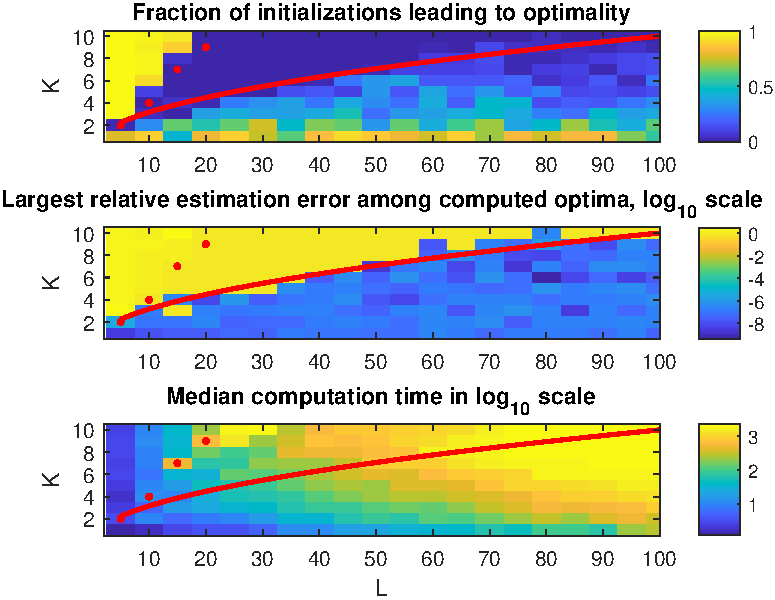
\includegraphics[width=.7\linewidth]{KLXP/XP1}
	\caption{In the $N \to \infty$ regime (access to exact moments, excluding biased entries) and with known uniform densities, it seems $K$ up to $\sqrt{L}$ (red curve) i.i.d.\ Gaussian signals of length $L$ can be recovered from the known moments. CPU time in seconds. Strictly above red dots, recovery is impossible because the number of unknowns exceeds the number of computed moments. Similar to~\cite[Fig.~4.1]{boumal2017heterogeneous}, this experiment suggests a possible statistical-computational gap.}
	\label{fig:KLXP}
\end{figure}


\section{Relation with cryo-EM + experiments?}
%
%In the simplified mathematical model above, we showed it is possible to estimate a signal without detecting its appearances.  
%Our strategy is to compute autocorrelations of the micrographs and to relate these statistics to the unknown signal's parameters. Recovering the parameters from the statistics reduces to solving a set of polynomial equations. 
%
%We also showed how this technique can, in principle, be applied to cryo-EM.
%Crucially, the outlined approach involves no particle picking, hence a fortiori no viewing direction estimation. Concerns for model bias are also greatly reduced since no template matching is involved.
%Additionally,  our technique also allows the use of much lower defocus values. Lower defocus means lower contrast, but will maintain  higher frequency information. Consequently, we may be able to get high resolution reconstructions from fewer micrographs.
%
%Looking toward applying the framework to encompass all important features of real cryo-EM experiments, our work implies that it might be possible to reconstruct small molecules, particularly, molecules that are too small to be detected in micrographs. 
%In pursuing this research direction, our goal is to significantly increase the range of molecules to which cryo-EM can be successfully applied.
%We recognize that significant challenges lay ahead for the implementation of the proposed approach to {high-resolution} 3-D reconstruction directly from the micrographs. We discuss a few now.
%
%The numerical experiments we have performed reveal that the third-order autocorrelation may not be enough for 3-D reconstruction in practice, due to high sensitivity.
%This suggests that fourth-order autocorrelation may be necessary. This in turn would imply that the procedure might require a large amount of data. 
%Recent trends in high-throughput cryo-EM technology   give hope that this may be a lesser concern in the long term. Still, large amounts of data also require large amounts of computation. On this front, we note that computing autocorrelations can be executed efficiently on CPUs and GPUs, and in parallel across micrographs. It can even be done in a  streaming mode, as only one pass through each micrograph is necessary. The output of this data processing stage is a summary in the form of autocorrelation estimates: its size is a function of the resolution, not a function of the number of observed micrographs. Subsequent steps, which involve solving the system of polynomial equations, scale only in the size of that summary. Of course, an important question then is whether the equations can be solved accurately and efficiently in practice. 
%
%To reach high-resolution reconstruction, beyond data acquisition and computational challenges, there are modeling issues  to consider.
%In contrast to the simplifying assumptions we have made above, the noise might be colored; the viewing directions of the particles may be distributed non-uniformly; there may be conformational heterogeneity; particles generally do not satisfy our separation condition; and micrographs undergo a contrast transfer function which we have omitted. All of these aspects can be handled with the same general strategy: establish a forward model relating the expected autocorrelations of the micrographs to the target volume(s) and all parameters necessary to model the above effects. 
%For instance, for colored noise, the forward model may involve multiple parameters to capture the power spectrum of the noise instead of the single parameter $\sigma^2$. 
%Similarly, instead of the separation condition, we can model the spacing between the projections using a parameterized pair-correlation function. Such a function models the distribution of distances between neighboring projections. The observed autocorrelations depend linearly on these parameters, which would be estimated as part of the inverse problem.
%All these aspects must be taken into account so the method can be applied on experimental data. We hope to take care of these issues in future research. 

%
%\section*{Acknowledgment}
%The authors  thank Ayelet Heimowitz, Joe Kileel,  Roy Lederman, Amit Moscovich, Nir Sharon and  Fred Sigworth for helpful discussions,  and Boris Landa and Yoel Shkolnisky for providing the code for the 2-D PSWFs expansion.
%The research was partially supported by Award Number R01GM090200 from the NIGMS, FA9550-17-1-0291 from AFOSR, Simons Foundation Math+X Investigator Award, and the Moore Foundation Data-Driven Discovery Investigator Award.
%NB is partially supported by NSF award DMS-1719558.

\bibliographystyle{plain}
\bibliography{ref}

\appendix

\section{Derivation of the identities in Section~\ref{sec:AC_analysis}} \label{sec:autocorrelation_computation}

We consider the asymptotic regime $N,M\to\infty$ and assume that $M=\Omega(N)$, so that
\begin{equation*}
\gamma := \frac{ML}{N}>0.
\end{equation*}
%
Any vectors with indices out of range are given value 0.
We focus here on the homogeneous model~\eqref{eq:model}. The extension to random signal $X$ is straight-forward by taking the expectation with respect to the distribution of $X$.

We start by considering the mean of the data:
\begin{equation*}
a_y^1 = \frac{1}{N}\sum_{i=0}^{N-1} y[i] =
\frac{1}{N/L}\sum_{j=0}^{M-1}\frac{1}{L}\sum_{i=0}^{L-1}x[i] +    
\underbrace{\frac{1}{N}\sum_{i=0}^{N-1}\varepsilon[i]}_{\text{noise term}}
\xrightarrow{a.s.}\gamma a_x^1,
\end{equation*}
%
where the noise term converges to zero almost surely (a.s.)\ by the strong law of large numbers.

We proceed with the (second-order) autocorrelation for fixed $\ell\in[0,\ldots,L-1]$. We can compute:
%
\begin{align*}
%
a_y^2[\ell] & = \frac{1}{N}\sum_{i=0}^{N-1-\ell}y[i]y[i+\ell]
\nonumber \\
& = \underbrace{\frac{1}{N}\sum_{j=1}^{M}\sum_{i=0}^{L-\ell-1}x[i]x[i+\ell]}_{\text{signal term}} + \underbrace{\frac{1}{N}\sum_{i=0}^{N-1-\ell}\varepsilon[i]\varepsilon[i+\ell]}_{\text{noise term}}
\\ & + \underbrace{\frac{1}{N} \sum_{j=1}^{M} \sum_{i=0}^{L-1} x[i] (\varepsilon[s_j + i + \ell] + \varepsilon[s_j + i - \ell])}_{\text{cross-term}}. 
%
\end{align*}
The cross-term is linear in the noise, and is easily shown to vanish almost surely in the limit $N\to\infty$, by the strong law of large numbers. We break the signal term into $M$ different sums, each containing one copy of the signal. This gives:
%
\begin{align} \label{eq:2nd_moment_signal_term}
%
\frac{1}{N}\sum_{j=1}^{M}\sum_{i=0}^{L-\ell-1}x[i]x[i+\ell] & = \frac{ML}{N}\frac{1}{L}\sum_{i=0}^{L-\ell-1}x[i]x[i+\ell]\nonumber\\&\xrightarrow{N\to\infty}\gamma a_x^2[\ell].
%
\end{align}
%
We next analyze the pure noise term. When $\ell\neq 0$, we can break the noise term into a sum of independent terms:
%
\begin{equation*}
%
\frac{1}{N}\sum_{i=0}^{N-1-\ell} \varepsilon[i]\varepsilon[i+\ell] = \frac{1}{\ell}\sum_{i=0}^{\ell-1}\frac{1}{N/\ell}\sum_{j=0}^{N/\ell -2} \varepsilon[j\ell + i] \varepsilon[(j+1)\ell + i].
%
\end{equation*}
%
Each sum $\frac{1}{N/\ell}\sum_{j=0}^{N/\ell -2} \varepsilon[j\ell + i] \varepsilon[(j+1)\ell + i]$ is an average of $N/\ell$ independent terms with expectation zero, hence converges to zero almost surely as $N\to\infty$. If $\ell=0$, then we have:
%
\begin{equation*}
\frac{1}{N}\sum_{i=0}^{N-1} \varepsilon^2[i] \xrightarrow{a.s.} \sigma^2.
\end{equation*}

We now analyze the third-order autocorrelation. Let us fix $\ell_1\geq\ell_2\ge0$. We have:
%
%\begin{align*}
%%
%&a_y^3[\ell_1,\ell_2] 
%= \frac{1}{N}\sum_{i=0}^{N-1-\ell_1} y[i]y[i+\ell_1]y[i+\ell_2]
%\nonumber \\
%%
%=& \underbrace{ \frac{ML}{N}\frac{1}{M}\sum_{j=1}^M 
%	\frac{1}{L}\sum_{i=0}^{L-1-\ell_1}x[i]x[i+\ell_1]x[i+\ell_2]   }_{(1)}
%\\& + \underbrace{\frac{1}{N}\sum_{i=0}^{N-1-\ell_1} \ep[i]\ep[i+\ell_1]\ep[i+\ell_2]}_{(2)}
%\nonumber \\
%&+ \underbrace{\frac{1}{N}\sum_{j=1}^{M} 
%	\sum_{i=0}^{L-1} x[i]\ep[s_j + i+\ell_1]\ep[s_j+ i+\ell_2]}_{(3)}
%\\& + \underbrace{\frac{1}{N}\sum_{j=1}^{M} 
%	\sum_{i=0}^{L-1} \ep[s_j+i-\ell_1]x[i]\ep[s_j+ i+\ell_2-\ell_1]}_{(4)}
%\nonumber \\
%&+ \underbrace{\frac{1}{N}\sum_{j=1}^{M} 
%	\sum_{i=0}^{L-1} \ep[s_j+i-\ell_2]\ep[s_j+i+\ell_1-\ell_2]x[i]}_{(5)}
%\\ & + \underbrace{\frac{1}{N}\sum_{j=1}^{M} 
%	\sum_{i=0}^{L-\ell_1+\ell_2-1} \ep[s_j+i-\ell_2]x[i+\ell_1-\ell_2]x[i]}_{(6)}
%\nonumber \\
%&+ \underbrace{\frac{1}{N}\sum_{j=1}^{M} 
%	\sum_{i=0}^{L-\ell_2-1} x[i]\ep[s_j + i+\ell_1]x[i+\ell_2]}_{(7)}
%\\ & + \underbrace{\frac{1}{N}\sum_{j=1}^{M} 
%	\sum_{i=0}^{L-\ell_1-1} x[i]x[i+\ell_1]\ep[s_j+ i+\ell_2]}_{(8)}.
%%
%\end{align*}
%
\begin{align*}
%
a_y^3[\ell_1,\ell_2] 
=& \frac{1}{N}\sum_{i=0}^{N-1-\ell_1} y[i]y[i+\ell_1]y[i+\ell_2]
\\
%
=& \underbrace{ \frac{ML}{N}\frac{1}{M}\sum_{j=1}^M 
	\frac{1}{L}\sum_{i=0}^{L-1-\ell_1}x[i]x[i+\ell_1]x[i+\ell_2]   }_{(1)}
+ \underbrace{\frac{1}{N}\sum_{i=0}^{N-1-\ell_1} \ep[i]\ep[i+\ell_1]\ep[i+\ell_2]}_{(2)}
\ \\
&+ \underbrace{\frac{1}{N}\sum_{j=1}^{M} 
	\sum_{i=0}^{L-1} x[i]\ep[s_j + i+\ell_1]\ep[s_j+ i+\ell_2]}_{(3)}
+ \underbrace{\frac{1}{N}\sum_{j=1}^{M} 
	\sum_{i=0}^{L-1} \ep[s_j+i-\ell_1]x[i]\ep[s_j+ i+\ell_2-\ell_1]}_{(4)}
\\
&+ \underbrace{\frac{1}{N}\sum_{j=1}^{M} 
	\sum_{i=0}^{L-1} \ep[s_j+i-\ell_2]\ep[s_j+i+\ell_1-\ell_2]x[i]}_{(5)}
+ \underbrace{\frac{1}{N}\sum_{j=1}^{M} 
	\sum_{i=0}^{L-\ell_1+\ell_2-1} \ep[s_j+i-\ell_2]x[i+\ell_1-\ell_2]x[i]}_{(6)}
\\
&+ \underbrace{\frac{1}{N}\sum_{j=1}^{M} 
	\sum_{i=0}^{L-\ell_2-1} x[i]\ep[s_j + i+\ell_1]x[i+\ell_2]}_{(7)}
+ \underbrace{\frac{1}{N}\sum_{j=1}^{M} 
	\sum_{i=0}^{L-\ell_1-1} x[i]x[i+\ell_1]\ep[s_j+ i+\ell_2]}_{(8)}.
%
\end{align*}
Terms (6), (7) and (8) are linear in $\ep$, and can easily be shown to converge to 0 almost surely by the law of large numbers, by similar arguments as used previously. Term (1) converges to $\gamma a_x^3[\ell_1,\ell_2]$ almost surely, for the same reasons as~\eqref{eq:2nd_moment_signal_term}. To deal with terms (2)--(5), we must distinguish between different values of $\ell_1$ and $\ell_2$.

{\bf Case 1:} $0 < \ell_2 < \ell_1$. Here, all summands with elements of $\ep$ involve products of distinct entries, which have expected value 0. Consequently, the usual argument shows that terms (2)--(5) all converge to 0 almost surely as $N \to \infty$.

{\bf Case 2:} $0=\ell_2 < \ell_1$. Term (2) is an average of products of the form $\ep[i]^2\ep[i+\ell_1]$, which have mean zero; consequently, term (2) converges to 0 almost surely. The same argument as for Case 1 shows that (3) and (5) also converge to 0. For term (4), we write:
%
\begin{align*}
%
&\frac{1}{N}\sum_{j=1}^{M} 
\sum_{i=0}^{L-1} \ep[s_j+i-\ell_1]x[i]\ep[s_j+ i+\ell_2-\ell_1]
\nonumber \\
&= \frac{ML}{N}\frac{1}{L}\sum_{i=0}^{L-1}x[i] \frac{1}{M}\sum_{j=1}^{M} \ep[s_j+i-\ell_1]^2
\\& \xrightarrow{a.s.} \gamma \frac{1}{L} \sum_{i=0}^{L-1}x[i] \sigma^2 = \gamma a_x^1 \sigma^2. \nonumber
%
\end{align*}

{\bf Case 3:} $0<\ell_2 = \ell_1$. An argument nearly identical to that for Case 2 shows that terms (2), (4) and (5) converge to 0, while term (3) converges to $\gamma a_x^1 \sigma^2$.

{\bf Case 4:} $0=\ell_2 = \ell_1$. The same argument as for term (4) in Case 2 shows that terms (3), (4) and (5) all converge to $\gamma a_x^1 \sigma^2$. Term (2) is an average of $\ep[i]^3$, which is mean zero; consequently, it converges to 0.
This completes the proof.


\section{Proof of Proposition~\ref{prop:gamma}} \label{sec:proof_prop_gamma}

In the limit, 
\begin{equation*}
(a^1_y)^2=\frac{\gamma^2}{L^2}\sum_{i=0}^{L-1}\sum_{j=0}^{L-1}x[i]x[j].
\end{equation*}
Similarly,  
\begin{equation*}
\sum_{\ell = 1}^{L-1}a_y^2[\ell]=\frac{\gamma}{L}\sum_{\ell = 1}^{L-1}\sum_{i=0}^{L-1-\ell}x[i]x[i+\ell],
\end{equation*}
and $a_y^2[0]=\frac{\gamma}{L}\sum_{i=0}^{L-1}x^2[i] + \sigma^2$. The proof is concluded by noting that  $a_x^2[-\ell]=a_x^2[\ell]$. 


\section{Proof of Proposition~\ref{prop:gamma_sigma}} \label{sec:proof_prop_gamma_sigma}

We prove that both $\sigma$ and $\gamma$ are identifiable from the observed first three moments of $y$. For convenience, we work with $\beta = \gamma / L$ rather than $\gamma$ itself. To this end, we construct two quadratic equations satisfied by $\beta$ and whose coefficients can be computed from observable quantities (in the limit). Then, we show that these equations are independent, and hence that $\beta$ is uniquely defined. Given $\beta$, we can estimate $\sigma$ using Proposition~\ref{prop:gamma}.

Throughout the proof, it is important to distinguish between observed and unobserved values.
We denote the observed values by $E_i$ or $a_y^1,a_y^2,a_y^3$. We use $F_i$ to denote functions of the signal's autocorrelations (which are not directly observable).

In the limit $N \to \infty$, almost surely, $a_y^1 = \beta(\one^Tx)$ and $a_y^2[0] = \beta\|x\|^2+\sigma^2$, where $\one\in\RL$ is the vector of all-ones. (In this whole section, for clarity, we now omit to specify that identities hold almost surely in the limit.) Consider the product:
\begin{equation}\label{eq:E1}
\begin{split}
E_1 := a_y^1a_y^2[0] =  (\beta(\one^Tx))(\beta\|x\|^2+\sigma^2)  = \sigma^2a_y^1 + L\beta^2F_1,
\end{split}
\end{equation}
where $F_1 := a_x^3[0,0] + \sum_{j=1}^{L-1}(a_x^3[j,j] + a_x^3[0,j])$. 
% Nicolas: the expression for F_1 is correct, see identifiability_of_gamma_and_sigma_Sep4_2018.m and notes Sep 4, 2018
The terms of $F_1$ can also be estimated from $a_y^3$, while taking the scaling and bias terms into account. This yields another observable:
\begin{align} 
E_2 & := a_y^3[0,0] + \sum_{j=1}^{L-1}(a_y^3[j,j] + a_y^3[0,j]) \nonumber\\
& = L\beta F_1 + (2L+1)\sigma^2a_y^1. \label{eq:E2}
\end{align}
% Nicolas: checked this one too.
Therefore, from~\eqref{eq:E1} and~\eqref{eq:E2} we get:
\begin{equation} \label{eq:E12}
E_2\beta -(2L+1)\sigma^2\beta a_y^1 = E_1-\sigma^2a_y^1.
\end{equation}
Let $E_3:=a_y^2[0] + 2\sum_{j = 1}^{L-1}a_y^2[j]$; recall from Proposition~\ref{prop:gamma}:
\begin{equation} \label{eq:sigma2}
\sigma^2 = E_3 - (a^1_y)^2/\beta. 
\end{equation} 
Plugging into~\eqref{eq:E12} and rearranging, we get a first quadratic equation in $\beta$,
\begin{equation} \label{eq:quad1}
\mathcal{A}\beta^2 + \mathcal{B}\beta + \mathcal{C} = 0,
\end{equation}
where 
\begin{align*}
\mathcal{A} &= E_2 - (2L+1)a_y^1E_3, \\ 
\mathcal{B} &= -E_1 + (2L+1)(a_y^1)^3 + a_y^1E_3  , \\
\mathcal{C} &= -(a_y^1)^3.
\end{align*}
Importantly, these coefficients are observable quantities. As we assume throughout this proof that $x$ has nonzero mean, $a_y^1 \neq 0$ and we conclude that this equation is non-trivial.

Next, we derive the second quadratic equation for $\beta$. We notice that 
\begin{equation} \label{eq:E3}
E_4 := \frac{1}{L}(a_y^1)^3 = \frac{1}{L}\beta^3 (\one ^Tx)^3   = \beta^3 F_2,
\end{equation}
where $F_2 = \frac{1}{L}(\one ^Tx)^3$, and we can work out that:
\begin{equation*}
F_2 = a_x^3[0,0] + 3\sum_{j=1}^{L-1} \left(a_x^3[j,j] + a_x^3[0,j]\right) + 6\sum_{1\leq i < j\leq L-1}a_x^3[i,j].
\end{equation*}
Once again, $F_2$ can be estimated from $a_y^3$, taking bias and scaling into account:
\begin{align}
E_5 & := a_y^3[0,0] + 3\sum_{j=1}^{L-1} \left(a_y^3[j,j] + a_y^3[0,j]\right) + 6\sum_{1\leq i < j\leq L-1}a_y^3[i,j]  = L \beta F_2 + (6L-3)\sigma^2a_y^1.
\end{align}
Consider the following ratio:
\begin{equation*} 
\frac{E_5}{E_4} = \frac{L}{\beta^2} + \frac{(6L-3)\sigma^2a_y^1}{E_4}.
\end{equation*}
From the latter, we deduce:
\begin{equation*}
\sigma^2 = \frac{E_5}{a_y^1(6L-3)}  - \frac{LE_4}{\beta^2a_y^1(6L-3)}.
\end{equation*}
Using~\eqref{eq:sigma2} and rearranging, we get the second quadratic:
\begin{equation} \label{eq:quad2}
\mathcal{D}\beta^2 + \mathcal{E}\beta + \mathcal{F} = 0,
\end{equation}
where
\begin{align*}
\mathcal{D} &= E_3 - \frac{E_5}{a_y^1(6L-3)}, \\ 
\mathcal{E} &= -(a_y^1)^2, \\
\mathcal{F} &= \frac{LE_4}{a_y^1(6L-3)}.
\end{align*}
It is also non-trivial since $E_4 \neq 0$.

To complete the proof, we need to show that the two quadratic equations~\eqref{eq:quad1} and~\eqref{eq:quad2} are independent. To this end, it is enough to show that the ratios between coefficients differ. 
From~\eqref{eq:quad1} and~\eqref{eq:E1}, we have:
\begin{equation*}
\begin{split}
\frac{\mathcal{B}}{\mathcal{C}} = \frac{E_1 - (2L+1)(a_y^1)^3 - a_y^1E_3}{(a_y^1)^3} = \frac{a_y^2[0] - (2L+1)(a_y^1)^2 - E_3}{(a_y^1)^2}.
\end{split}
\end{equation*}
In addition, using~\eqref{eq:E3},
\begin{equation*}
\frac{\mathcal{E}}{\mathcal{F}} = \frac{(3-6L)(a_y^1)^3}{LE_4} = 3 - 6L . 
\end{equation*}
For contradiction, suppose that the quadratics are dependent. Then, $\frac{\mathcal{B}}{\mathcal{C}} =\frac{\mathcal{E}}{\mathcal{F}} $, that is, 	
\begin{equation*}
a_y^2[0] - (2L+1)(a_y^1)^2 - E_3 = (a_y^1)^2(3-6L).
\end{equation*}
Rewriting the identity in terms of $x$ and dividing by $\beta$ we get:
\begin{equation} \label{eq:cond}
4(L-1)\beta (\1^\top x)^2  - (\1^\top x)^2 + \|x\|^2 = 0.
\end{equation}	
For generic $x$,  this polynomial equation is not satisfied so that the quadratic equations are independent. 
Furthermore, from the inequality $L\|x\|^2 \ge (\1^\top x)^2$ it follows immediately that the equations must be independent so long as
\begin{equation*}
\beta > \frac{1}{4L}.
\end{equation*}

\section{Proof of Proposition~\ref{prop:poisson}} \label{sec:proof_prop_poisson}


\subsection{First moment}

To compute the first moment of $y$, we will first condition on $M = (M_1,\dots,M_{N-L+1})$, and then average over $M$. We have:
%
\begin{align}
%
\E[y[i] | M] = \sum_{j=0}^{L-1} \sum_{k=1}^{M_{i-j}} \E X_k^{i-j}[j]
= \sum_{j=0}^{L-1} \sum_{k=1}^{M_{i-j}} m_y^1[j]
= \sum_{j=0}^{L-1} M_{i-j} m_y^1[j].
%
\end{align}
%
Now taking expectations over $M$ we see:
%
\begin{align}
%
\E Y[i] = \gamma \sum_{j=0}^{L-1}  m_y^1[j] = \gamma La_x^1.
%
\end{align}


%


\subsection{Second moment}

Again, we will condition on $M$ first, and then take the expectation over $M$. Fix $i_1 \ne i_2$, and let $\Delta = i_2 - i_1$. Then:
%
\begin{align}
%
Y_{i_1} Y_{i_2} 
&= \sum_{j_1=0}^{L-1} \sum_{j_2=0}^{L-1} 
\sum_{k_1=1}^{M_{i_1-j_1}}\sum_{k_2=1}^{M_{i_2-j_2}}
X_{k_1}^{i_1-j_1}[j_1] X_{k_2}^{i_2 - j_2}[j_2].
%
\end{align}

We break up the double sum over $j_1$ and $j_2$ into two terms: one where $j_2 \ne j_1 + \Delta$, and one where $j_2 = j_1 + \Delta$ or equivalently $i_1-j_1 = i_2-j_2$. In the first case, all the terms are independent, and so the expectation factors. In the second case, when $k_1 \ne k_2$ we have independence, but otherwise not. This gives (all expectations are conditional on $M$):
%
\begin{align} \label{moment2-condm}
%
\E Y_{i_1} Y_{i_2}
=& \sum_{j_1=0}^{L-1} \sum_{j_2=0}^{L-1} 
\sum_{k_1=1}^{M_{i_1-j_1}}\sum_{k_2=1}^{M_{i_2-j_2}}
\E X_{k_1}^{i_1-j_1}[j_1] X_{k_2}^{i_2 - j_2}[j_2]
\nonumber \\
=& \sum_{j_1 - j_2 \ne \Delta} \sum_{k_1} 
\sum_{k_2} \E X_{k_1}^{i_1-j_1}[j_1] X_{k_2}^{i_2 - j_2}[j_2]
\nonumber \\
& + \sum_{j_1 = 0}^{L-1} \sum_{k_1 \ne k_2} 
\E X_{k_1}^{i_1-j_1}[j_1] X_{k_2}^{i_1 - j_1}[j_1+\Delta]
\nonumber \\
& + \sum_{j_1 = 0}^{L-1} \sum_{k_1=1}^{M_{i_1-j_1}} 
\E X_{k_1}^{i_1-j_1}[j_1] X_{k_1}^{i_1-j_1}[j_1 + \Delta] 
\nonumber \\
=& \sum_{j_1 - j_2 \ne \Delta} M_{i_1-j_1} M_{i_2 - j_2} \M_1[j_1] \M_1[j_2]
\nonumber \\
& + \sum_{j_1 = 0}^{L-1} M_{i_1-j_1}(M_{i_1-j_1} - 1) \M_1[j_1] \M_1[j_1 + \Delta]
\nonumber \\
& + \sum_{j_1 = 0}^{L-1} M_{i_1-j_1} \M_2[j_1,j_1 + \Delta] .
%
\end{align}
%
Now take expectations over the Poisson random variables, using this fact:
%
\begin{lem} \label{lem-choose}
	If $M \sim \Poisson(\gamma)$, then 
	\begin{align}
	%
	\E {M\choose k} = \frac{\gamma^k}{k!}.
	%
	\end{align}
\end{lem}


We get (now the expectation is over $M$ and $X$):
%
\begin{align}
%
\E Y_{i_1} Y_{i_2} 
=& \sum_{j_1 - j_2 \ne \Delta} \E M_{i_1-j_1} M_{i_2 - j_2} \M_1[j_1] \M_1[j_2]
\nonumber \\
& + \sum_{j_1 = 0}^{L-1} \E M_{i_1-j_1}(M_{i_1-j_1} - 1) \M_1[j_1] \M_1[j_1 + \Delta]
\nonumber \\
& + \sum_{j_1 = 0}^{L-1} \E M_{i_1-j_1} \M_2[j_1,j_1 + \Delta]
\nonumber \\
=& \sum_{j_1 - j_2 \ne \Delta} \gamma^2 \M_1[j_1] \M_1[j_2]
+ \sum_{j_1 = 0}^{L-1} \gamma^2 \M_1[j_1] \M_1[j_1 + \Delta]
\nonumber \\
& + \sum_{j_1 = 0}^{L-1} \gamma \M_2[j_1,j_1 + \Delta]
\nonumber \\
=&  \bigg(\gamma \sum_{j = 0}^{L-1} \M_1[j] \bigg)^2
+ \gamma \sum_{j = 0}^{L-1} \M_2[j,j + \Delta]
\nonumber \\
=&  (\gamma \L_1)^2 + \gamma \L_2(\Delta).
%
\end{align}

But the first term in the sum is just the square of the first moment of $Y$; so from the first two moments we can recover $\gamma \L_2(\Delta)$, which is just the expected power spectrum of the random vector $X$, i.e.\ the usual second moment we have been working with.


%


\subsection{Third moment}

For three distinct $i_1$, $i_2$ and $i_3$, we let $\Delta_1 = i_2 - i_1$ and $\Delta_2 = i_3 - i_1$. We have:
%
\begin{align}
%
&Y_{i_1} Y_{i_2} Y_{i_3}
\nonumber \\
&= \sum_{j_1=0}^{L-1} \sum_{j_2=0}^{L-1} \sum_{j_3=0}^{L-1} 
\sum_{k_1=1}^{M_{i_1-j_1}}\sum_{k_2=1}^{M_{i_2-j_2}} \sum_{k_3=1}^{M_{i_3-j_3}}
X_{k_1}^{i_1-j_1}[j_1] X_{k_2}^{i_2 - j_2}[j_2] X_{k_3}^{i_3 - j_3}[j_3].
\end{align}
%
We will break up the outer three sums into disjoint sums with the following ranges of indices:
%
\begin{enumerate}
	
	\item \label{case1}
	$j_2 = j_1 + \Delta_1$ and $j_3 = j_2 + \Delta_2 - \Delta_1$.
	
	\item \label{case2}
	$j_2 = j_1 + \Delta_1$ and $j_3 \ne j_2 + \Delta_2 - \Delta_1$.
	
	\item \label{case3}
	$j_2 \ne j_1 + \Delta_1$ and $j_3 = j_1 + \Delta_2$.
	
	\item \label{case4}
	$j_2 \ne j_1 + \Delta_1$ and $j_3 \ne j_1 + \Delta_2$ and $j_3 = j_2 + \Delta_2 - \Delta_1$.
	
	\item \label{case5}
	$j_2 \ne j_1 + \Delta_1$ and $j_3 \ne j_1 + \Delta_2$ and $j_3 \ne j_2 + \Delta_2 - \Delta_1$.
	
\end{enumerate}


For Case \ref{case1}, we have $\ell \equiv i_1 - j_1 = i_2 - j_2 = i_3 - j_3$. We further break up the sum:
%
\begin{align}
%
&\sum_{j=0}^{L-1} \sum_{k_1=1}^{M_\ell} \sum_{k_2=1}^{M_\ell} \sum_{k_3=1}^{M_\ell} 
X_{k_1}^{\ell}[j] X_{k_2}^{\ell}[j + \Delta_1] X_{k_3}^{\ell}[j + \Delta_2]
\nonumber \\
=& \underbrace{ \sum_{j=0}^{L-1} \sum_{k_i \text{distinct}} 
	X_{k_1}^{\ell}[j] X_{k_2}^{\ell}[j + \Delta_1] X_{k_3}^{\ell}[j + \Delta_2]
}_{\text{(a)}}
\nonumber \\
&+\underbrace{ \sum_{j=0}^{L-1} \sum_{k_1=k_2\ne k_3} 
	X_{k_1}^{\ell}[j] X_{k_2}^{\ell}[j + \Delta_1] X_{k_3}^{\ell}[j + \Delta_2]
}_{\text{(b)}}
\nonumber \\
&+\underbrace{ \sum_{j=0}^{L-1} \sum_{k_1=k_3\ne k_2} 
	X_{k_1}^{\ell}[j] X_{k_2}^{\ell}[j + \Delta_1] X_{k_3}^{\ell}[j + \Delta_2]
}_{\text{(c)}}
\nonumber \\
&+\underbrace{ \sum_{j=0}^{L-1} \sum_{k_2=k_3\ne k_1} 
	X_{k_1}^{\ell}[j] X_{k_2}^{\ell}[j + \Delta_1] X_{k_3}^{\ell}[j + \Delta_2]
}_{\text{(d)}}
\nonumber \\
&+\underbrace{ \sum_{j=0}^{L-1} \sum_{k_1=k_2=k_3} 
	X_{k_1}^{\ell}[j] X_{k_2}^{\ell}[j + \Delta_1] X_{k_3}^{\ell}[j + \Delta_2]
}_{\text{(e)}}.
%
\end{align}

For term (a), the expectation conditional on $M$ is:
%
\begin{align}
%
\sum_{j=0}^{L-1} M_\ell(M_\ell-1)(M_\ell-2)\M[j] \M[j+\Delta_1] \M[j+\Delta_2].
%
\end{align}
%
Using Lemma \ref{lem-choose}, the unconditional expectation of (a) is then:
%
\begin{align} \label{aaaa}
%
\gamma^3 \sum_{j=0}^{L-1} \M_1[j] \M_1[j+\Delta_1] \M_1[j+\Delta_2].
%
\end{align}


For term (b), the expectation conditional on $M$ is:
%
\begin{align}
%
\sum_{j=0}^{L-1} M_\ell (M_\ell - 1) \M_2[j,j+\Delta_1] \M_1[j + \Delta_2]
%
\end{align}
%
and then again using Lemma \ref{lem-choose} we get the expected value:
%
\begin{align} \label{bbbb}
%
\gamma^2 \sum_{j=0}^{L-1} \M_2[j,j+\Delta_1] \M_1[j+\Delta_2].
%
\end{align}

Similarly, the expected values of terms (c) and (d) are:
%
\begin{align} \label{cccc}
%
\gamma^2 \sum_{j=0}^{L-1} \M_2[j,j+\Delta_2] \M_1[j+\Delta_1].
%
\end{align}
%
and
%
\begin{align} \label{dddd}
%
\gamma^2 \sum_{j=0}^{L-1} \M_2[j+\Delta_1,j+\Delta_2] \M_1[j].
%
\end{align}

Finally, the expected value of term (e) is easily shown to be:
%
\begin{align} \label{eeee}
%
\gamma \sum_{j=0}^{L-1} \M_3[j,j+\Delta_1,j+\Delta_2].
%
\end{align}
%
This concludes the computation for Case \ref{case1}.

Moving onto Case \ref{case2}, we have $\ell_1 \equiv i_1 - j_1 = i_2 - j_2$, and also define $\ell_2 \equiv i_3 - j_3$. By definition, $\ell_1 \ne \ell_2$. The sum is:
%
\begin{align}
%
& \sum_{j_1=0}^{L-1} \sum_{j_3 \ne j_1 + \Delta_2}
\sum_{1 \le k_1,k_2 \le M_{\ell_1}} \sum_{k_3=1}^{M_{\ell_2}}
X_{k_1}^{\ell_1}[j_1] X_{k_2}^{\ell_1}[j_1 + \Delta_1] X_{k_3}^{\ell_2}[j_3]   
\nonumber \\
=& \sum_{j_1=0}^{L-1} \sum_{j_3 \ne j_1 + \Delta_2} \sum_{k_3=1}^{M_{\ell_2}}
\Bigg\{
\sum_{1 \le k_1 \ne k_2 \le M_{\ell_1}} 
X_{k_1}^{\ell_1}[j_1] X_{k_2}^{\ell_1}[j_1 + \Delta_1] X_{k_3}^{\ell_2}[j_3]
\nonumber \\
&       + \sum_{k_1=1}^{M_{\ell_1}} X_{k_1}^{\ell_1}[j_1] X_{k_1}^{\ell_1}[j_1 + \Delta_1] 
X_{k_3}^{\ell_2}[j_3]  \Bigg\}.
%
\end{align}
%
Taking expectations conditional on $M$, we then get:
%
\begin{align}
%
& \sum_{j_1=0}^{L-1} \sum_{j_3 \ne j_1 + \Delta_2} 
\Bigg(M_{\ell_1} (M_{\ell_1}-1) M_{\ell_2} \M_1[j_1] \M_1[j_1 + \Delta_1] \M_1[j_3]
\nonumber \\
&       + M_{\ell_1} M_{\ell_2} \M_2[j_1,j_1+\Delta_1] \M_1[j_3] \Bigg).
%
\end{align}

Taking expectations over $M$ and using Lemma \ref{lem-choose} then gives:
%
\begin{align}
%
& \gamma^3 \sum_{j_1=0}^{L-1} \sum_{j_3 \ne j_1 + \Delta_2} 
\M_1[j_1] \M_1[j_1 + \Delta_1] \M_1[j_3]
\label{ffff} \\
& + \gamma^2 \sum_{j_1=0}^{L-1} \sum_{j_3 \ne j_1 + \Delta_2}  
\M_2[j_1,j_1+\Delta_1] \M_1[j_3].
\label{gggg}
%
\end{align}


Similarly, Cases \ref{case3} and \ref{case4} give the expressions:
%
\begin{align}
%
& \gamma^3 \sum_{j_1=0}^{L-1} \sum_{j_2 \ne j_1 + \Delta_1} 
\M_1[j_1] \M_1[j_1 + \Delta_2] \M_1[j_2]
\label{hhhh} \\
& + \gamma^2 \sum_{j_1=0}^{L-1} \sum_{j_2 \ne j_1 + \Delta_1}  
\M_2[j_1,j_1+\Delta_2] \M_1[j_2]
\label{iiii}
%
\end{align}
%
and
%
\begin{align}
%
& \gamma^3 \sum_{j_2=0}^{L-1} \sum_{j_1 \ne j_2} 
\M_1[j_1] \M_1[j_2 + \Delta_1] \M_1[j_2 + \Delta_2]
\label{jjjj}\\
& + \gamma^2 \sum_{j_2=0}^{L-1} \sum_{j_1 \ne j_2}  
\M_2[j_2+\Delta_1,j_2+\Delta_2] \M_1[j_1].
\label{kkkk}
%
\end{align}

Finally, in Case \ref{case5} we have $i_1 - j_1$, $i_2 - j_2$, and $i_3 - j_3$ are all pairwise distinct. Consequently, the $X$ variables are always independent, and the expectation conditional on $M$ (letting $\ell_q = i_q - j_q$, $q=1,2,3$),
%
\begin{align}
%
\sum_{j_1,j_2,j_3} M_{\ell_1} M_{\ell_2} M_{\ell_3} \M_1[j_1] \M_1[j_2] \M_1[j_3];
%
\end{align}
%
since the $M_{\ell_q}$'s are pairwise independent, $q=1,2,3$, the expectation over $M$ then yields:
%
\begin{align} \label{llll}
%
\gamma^3 \sum_{j_1,j_2,j_3} \M_1[j_1] \M_1[j_2] \M_1[j_3].
%
\end{align}

Now we add all the terms from Cases \ref{case1} to \ref{case5}. Expressions \eqref{aaaa}, \eqref{ffff}, \eqref{hhhh}, \eqref{jjjj}, and \eqref{llll} sum to the expression:
%
\begin{align}
%
(\gamma \L_1)^3.
%
\end{align}

Note that this is obtained directly from the first moment. Expressions \eqref{bbbb}, \eqref{cccc}, \eqref{dddd}, \eqref{gggg},\eqref{iiii}, and \eqref{kkkk} sum to the expression:
%
\begin{align}
%
\gamma \L_1  \cdot 
( \gamma\L_2(\Delta_1) + \gamma\L_2(\Delta_2) + \gamma\L_2(\Delta_2-\Delta_1)).
%
\end{align}
%
Again, note that this is obtained directly from the first two moments. Finally, expression \eqref{eeee} is simply:
%
\begin{align}
%
\gamma \L_3(\Delta_1,\Delta_2)
%
\end{align}
%
which is the usual third-order auto-correlation.


\end{document}


